% Source: Wald GR, physical PDF p. 426
%         (printed p. 413).
% Coverage: Collapse followed by complete black-hole evaporation.
% Figures/tables/footnotes: Figure 14.4; no tables or footnotes.
% Status: source-reviewed and compile-clean.
% Uncertainties: none.

\begingroup
\renewcommand{\thefigure}{14.4}
\begin{figure}[htbp]
  \centering
  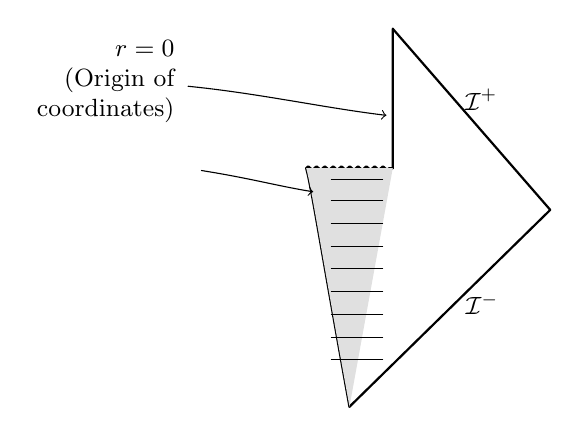
\begin{tikzpicture}[x=1cm,y=1cm,font=\small,line cap=round,line join=round]
    \coordinate (B) at (0,-2.35);
    \coordinate (R) at (2.55,.15);
    \coordinate (T) at (.55,2.45);
    \coordinate (S) at (.55,.68);
    \coordinate (C) at (-.55,.68);
    \draw[thick] (B)--(R)--(T)--(S);
    \draw[thick] (S)--(T);
    \draw[thick,decorate,decoration={zigzag,segment length=3pt,amplitude=.65pt}]
      (C)--(S);
    % Surface of the collapsing matter and shaded black-hole region.
    \draw[thick] (B) .. controls (-.38,-.25) and (-.48,.42) .. (C);
    \path[fill=black!12] (B) .. controls (-.38,-.25) and (-.48,.42) .. (C)
      -- (S) -- cycle;
    \foreach \yy in {-1.75,-1.47,-1.18,-.89,-.60,-.31,-.02,.27,.54}
      \draw[thin] (-.23,\yy)--(.42,\yy);
    \draw[->] (-2.05,1.72) .. controls (-1.15,1.63) and (-.35,1.45) .. (.47,1.35);
    \draw[->] (-1.88,.65) .. controls (-1.25,.55) and (-.90,.45) .. (-.46,.38);
    \node[left,align=right] at (-2.10,1.78) {\(r=0\)\\(Origin of\\coordinates)};
    \node[right] at (1.34,1.55) {\(\mathcal I^+\)};
    \node[right] at (1.35,-1.05) {\(\mathcal I^-\)};
  \end{tikzpicture}
  \caption{A conformal diagram of a spacetime in which a black hole is produced
  by the collapse of matter and ``evaporates'' as a result of the particle creation
  process.}
  \label{fig:14.4}
\end{figure}
\endgroup
